\chapter{Былина о Добрыне и Змее}

Целых два киевских предания связаны со «змиями» с Кирилловских высот, с легендарной пещерой. Обычно вспоминают легенду о Никите Кожемяке или Кирилле Кожемяке – как его звали на самом деле, неведомо.

Но мы начнем с другой истории, с былин о Добрыне Никитиче и Змие. Былины – для рассуждений зыбкая почва. Существует множество вариантов описания одного и того же события. Что в них общее, то основа. А разница – то или выдумка сказителя, или правдивое уточнение, и черт разберет, как понимать. 

Рассказчики былин сокращали и добавляли. Например, трехпудовый шлем Добрыни, коим богатырь дерется со змеем, менее правдоподобен, чем тот же шлем, однако наполненный тремя пудами песка, а это около пятидесяти кило.

Общее же у былин – место действия, и зря многие исследователи распределяют окрестности Киева, упомянутые в былинах «киевского цикла», по другим местам, перенося одно на Урал, другое еще куда. В былинах, киевские местности приведены в правильном взаимном географическом отношении. Это важно.

Конечно, без изменений сказание, передаваемое былиной, из прошлого в настоящее дойти не могло. Личность сказителя – откуда он родом, цепкость памяти, склонность к сочинительству – накладывала на былину отпечаток, искажая её.

Некоторые составители сборников былин занимались правкой, устраняя так называемые «анахронизмы» – например, выкидывали из текстов упоминания про огнестрельное оружие, подзорные трубы (после такой дурной правки богатыри смотрят в кулаки), а также дополняли по своему усмотрению, играясь в поэтов. 

Этим сильно грешат сборники Авенариуса. Мало того, что Авенариус произвольно правил былины, но еще вклинивал туда сюжетную линию, в коей «загусельник» Добрыня время от времени поет перед другими богатырями короткие былины. 

Поэтому если изучать былины, то за предмет изучения следует брать те исходники, которые были предоставлены собирателями вроде Гильфердинга.

Знание истории помогает понять тексты былин. Например, урочище «Леванидов чудный крест» – это крест, взятый князем Владимиром из Корсуня (Херсонеса), где Владимира крестили. Леванидовый – от епископа Левонтия. После, крест поставили в Киеве, «на лугах», которые и получили название лугов Леванидовых. А вот где они находились – загадка.

Добрыня по сведениям летописи был вуем, дядей князя Владимира («И бе Добрыня уй Володимерю, мать его бе сестра Добрынина»). Некоторые сказители былин называли Добрыню племянником Владимира. По былинам же, Добрыня не княжеского роду, но боярского, что служило препятствием к его женитьбе на племяннице Владимира, Забаве Путятичне. Добрыня-сподвижник Владимира из летописи, и Добрыня из былин – один человек или разные?

Разные, у них отчество разное. Былинный – Никитич, а летописный – сын Малка Любечанина.

Существует много вариантов былины о Добрыне и змее. Ниже попытаюсь свести их воедино и кратко изложить.

В Киеве или около, с матушкой своей, в палатах белокаменных, жил Добрыня Никитич. Жарким днем он надумал поехать через чисто поле (чем не Оболонь?) купаться на Пучай-реку, Пучайку. Конечно же, это Почайна! Пучай-река около Киева упомянута и в былине о Дюке Степановиче, где богатыри соревнуются, прыгая через Пучай на своих богатырских конях с «подкрылышками подкожными», причем чем больше этих подкрылышков имел конь, тем дальше мог прыгнуть – через половину реки, через всю реку и так далее.

Возле реки была некая «гора Сорочинская». Это один из холмов Кирилловских высот, либо они все. Сорочинская то же, что Сарацинская, а на Кирилловских высотах найдены были клады арабских монет, да и наличие района Татарки в верховьях высот нельзя оставить без внимания. 

Проверим, насколько справедливо мое сопоставление «Сорочинцев» с Востоком. Далеко ходить не надо. Поселок Большие Сорочинцы под Полтавой. В двадцати с копейками километрах от него есть деревня Дамаска. Близко и село Абаз, а ведь это слово обозначает старинную сирийскую монету. Восточное, мусульманское – что еще рядом с Большими Сорочинцами? Ордановка, Тахтаулово. В Орде «тахтаул» – воинский чин, близкий к престолу, а также татарское имя. Вместе с тем названия других деревень тоже указывают на народы, их основавшие – например Бессарабы, Волошковое. Население сердца Европы – земель нынешней Украины, где пересеклись все мыслимые торговые пути, было разнородно.

В местности с Пучай-рекой, полем, горой – обитала змея и змееныши\footnote{В статье Н. В. Шарлеманя 1965 года, «К вопросу о топонимике р. Почайны и попытка реалистического толкования былины «Добрыня и змей»» есть любопытные сведения о Почайне: «В наше время еще можно видеть речку Почайну и ее вершину, у которой и в древности, вероятно, был брод, где левый берег и ныне у местного населения называется Змієвате». Однако я не знаю, что подразумевал Шарлемань под вершиной Почайны.}. Змея брала в плен людей. В некоторых вариантах былины уточнение – «змея Горынчище». Стало быть, змея из горы. А живет она там в «пещерушках».

Зная опасность задуманного сыном, матушка отговаривает Добрыню, однако тот не слушается и отправляется к Пучай-реке, взяв с собой слугу-«паробка».

Разделся, стал купаться, говорит вслух – мол, река вовсе не бурная, а спокойная как лужа болотная. Далее случилось вот что:

\settowidth{\versewidth}{А и дождя то нет, да только гром гремит,} 
\begin{verse}[\versewidth]
Не успел Добрыня словца смолвити – \\
Ветра нет, да тучу нанесло,\\
Тучи нет, да будто дождь дождит,\\
А и дождя то нет, да только гром гремит,\\
Гром гремит да свищет молния\\
А как летит Змеище Горынище\\
О тыех двенадцати о хоботах.\\
А Добрыня той Змеи не приужахнется.\\
\end{verse}

Прервемся. Удивительно, как же проявления «змея» подобны проявлениям Перуна, бога грома и молнии! Без самоцензуры сказителей, вместо «змея» вполне может быть Перун.

И снова – Змеище Горынище. Змей из горы.
   
В варианте, опубликованном Миллером в «Былинах новой и недавней записи из разных местностей России» 1908 года, полет змея описан так:

\settowidth{\versewidth}{Вылетал-то тут змеинище-Горынище.} 
\begin{verse}[\versewidth]
Вылетал-то тут змеинище-Горынище.\\
Веют крылья его гумажныя,\\
Звенят его хоботы железные...\\
\end{verse}

Стало быть, крылья были сделаны из чего-то подобного бумаге, по крайней мере с виду. А хоботы значит железные и звенят. А нам твердят – дракон, дракон. Да летательный аппарат, а не рептилия. 

Один вариант былины прямо указывает, откуда прибывает змея – с западной стороны. То есть от Кирилловских высот, которые лежат к западу от Почайны.

\settowidth{\versewidth}{Похотелось тут молодому Добрынюшки} 
\begin{verse}[\versewidth]
Похотелось тут молодому Добрынюшки\\
Покупаться во Пучай реки, поныркати.\\
Там на тую пору, на то времецко\\
Да из далеча далече из чиста поля,\\
Из под западнёй да с под сторонушки, \\
\end{verse}

И далее, по прежнему варианту:

\settowidth{\versewidth}{Захочу тебя, Добрыня, теперь съем сожру,} 
\begin{verse}[\versewidth]
Говорит Змея ему проклятая:\\
Ты теперича, Добрыня, во моих руках!\\
Захочу тебя, Добрыня, теперь потоплю,\\
Захочу тебя, Добрыня, теперь съем сожру,\\
Захочу тебя, Добрыня, в хобота возьму,\\
В хобота возьму, Добрыня, во нору снесу!\\
\end{verse}

Хобота – что за хобота такие? Всегда прибегаем к тому, как разумели это слово в старину. Хоботом называли хвост. А такоже – рукав (насоса), нечто длинное для всасывания, и даже рычаг. А может, у змеи были подобные хоботам манипуляторы для подъема грузов. Но хобота еще и звенели. Может, словом «хобот» в различных былинах обозначали разные вещи.

Слуга Добрыни убегает, унося не токмо коня, но и оружие. Добрыня ныряет и выплывает у другого берега. Глядит на противоположный – пусто. Обороняться нечем. Думает – вот и всё. А «змея» начинает летать и жечь богатыря искрами.

Тут Добрыня замечает на бережке свой «колпак земли греческой». А это шлем вот такой формы:

\begin{center}
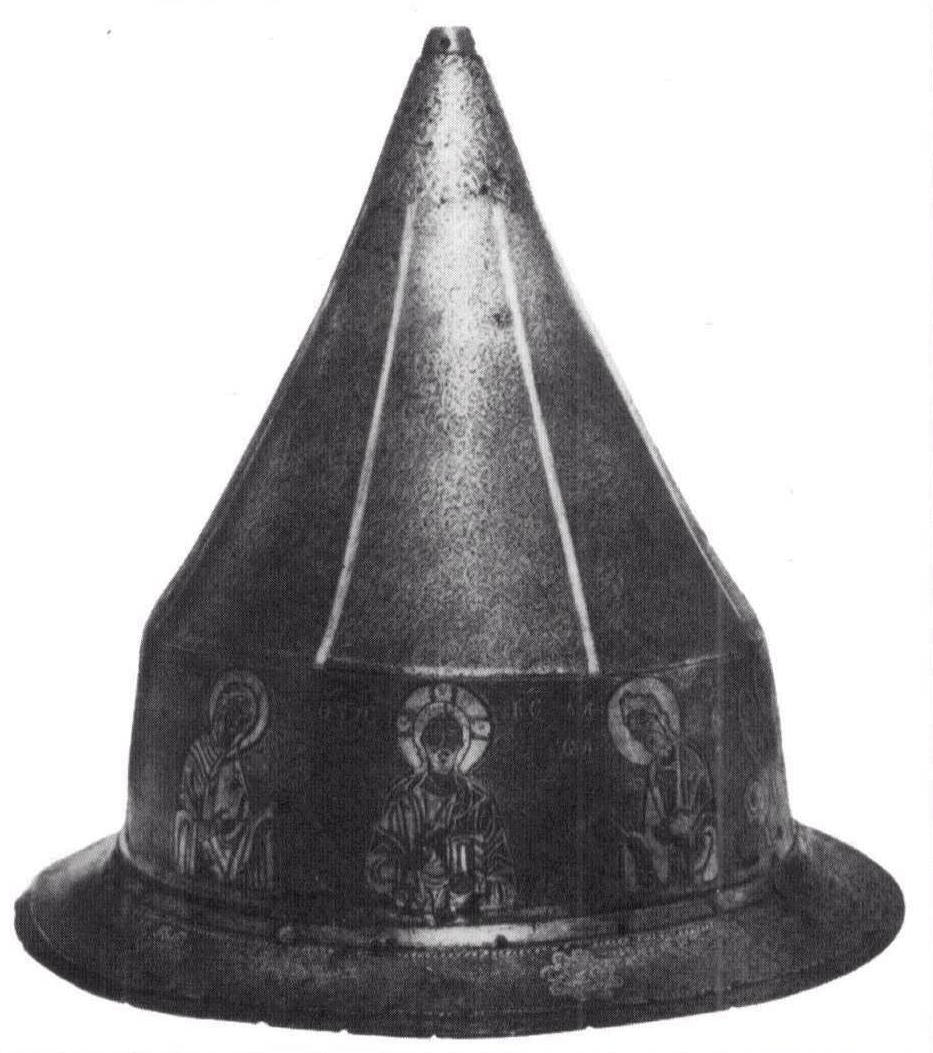
\includegraphics[width=0.60\linewidth]{chast-zmiy/dobrynya/kolpak-big.jpg}
\end{center}

В некоторых вариантах былины колпак весил три пуда, то есть 50 килограммов. В более полном варианте, шлем сей – обыкновенный, просто Добрыня набирает в него песок (те же три пуда), и этим утяжеленным шлемом отшибает змее не то три хобота, не то все. Змей падает на землю.

«Колпак» между прочим послужил ученым основой множеству споров, а в примечаниях к былине усердно пишут сноску, трактуя колпак то как «шапка паломника», то как «монашеский клобук». Я понимаю, если бы герои Печерского Патерика воевали клобуками, но светскому Добрыне более присущ именно шлем. Сказано было о нем – живет с матерью в палатах белокаменных, на гуслях играет, одевается витязем.

Даль поясняет, что в старину означало слово колпак: «шелом островерхий, с яблоком, репьем; шеломом звали  круглый  сверху, а шишаком высокий, с шишом (трубкою) и еловцем». Но часто упоминаемый в этой книге академик Рыбаков лихо рубит с плеча: «Эта шапка – монаший клобук, воплощающий веру в Христа». Да с чего вдруг?!

\begin{center}
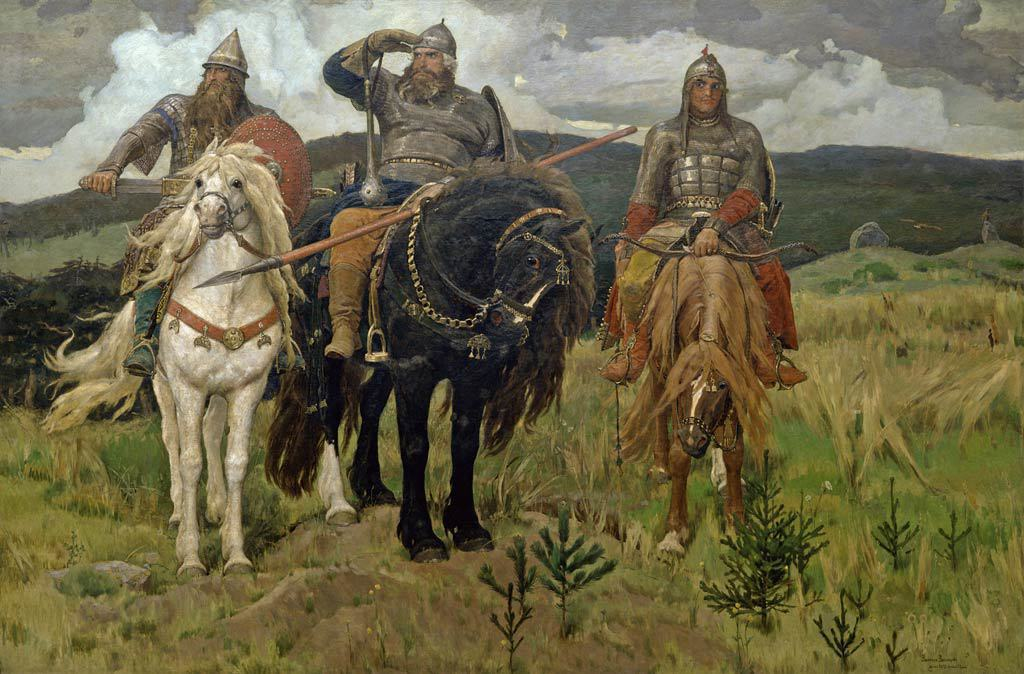
\includegraphics[width=\linewidth]{chast-zmiy/dobrynya/tri-bog-02.jpg}
\end{center}

Кстати, на картине Васнецова «Богатыри», над которой художник работал тридцать лет, Добрыня изображен именно в «колпаке земли греческой». Вот он, Добрыня, слева стоит.

Вернусь к изложению былины, в которой, полагаю, если отбросить узорчатые словесы, много и правды. Побежденная змея заключает с Добрыней договор – Никитич не суется в её владения, а она больше не летает на святую Русь и не похищает людей:

\settowidth{\versewidth}{Не купаться ти, Добрыне, во Пучай-реке.} 
\begin{verse}[\versewidth]
«Ах ты, ай, Добрыня сын Никитинец!\\
Мы положим с тобой заповедь великую:\\
Тебе не ездити далече во чисто поле,\\
На тую на гору сорочинскую,\\
Не топтать больше младыих змеенышей,\\
А не выручать полонов да русскиих,\\
Не купаться ти, Добрыне, во Пучай-реке.\\
И мне не летать да на святую Русь,\\
Не носить людей мне больше русскиих ,\\
Не копить мне полонов да русскиих».\\
\end{verse}

И Добрыня отпускает змею:

\settowidth{\versewidth}{Он повыпустил Змею как с под колен своих -} 
\begin{verse}[\versewidth]
Он повыпустил Змею как с под колен своих -\\
Поднялась Змея да вверх под облако.\\
\end{verse}

Долго ли, коротко, змея принимается за старое – на сей раз похищает человека, которого не следовало трогать – дочь князя Владимира. Когда простых людей уволакивала, это ей сходило с рук. А тут осечка.

Но Владимир не знает, что делать. Кого из придворных богатырей послать на выручку племяннице? Алёша Попович, недруг Добрыни, вечно его хочет куда-то сплавить, советует князю – вот мол, лучше Добрыни для этого не найти, у него и договоренность со змеей есть, так что вернет Забаву без кровопролития. Добрыня однако же сражается со змеем, побеждает его, и вызволяет из пещер томящихся там людей, а купно с ними и Забаву Путятичну, распятую гвоздями.

В некоторых вариантах былины названия мест разнятся. Так, в сборнике Кирши Данилова вместо Сорочинской горы – «Туги-гора».

«Туги» – не созвучно ли с «Тугариным»? В другом варианте Добрыня едет купаться на Сафат-реку вместо Пучай-реки. С этой Сафат-рекой тоже связан некий «Змеёвич». В былине про Алёшу Поповича (по отчеству Леонтьевич), на пути к Киеву, Алёша и Еким Иванович:

\settowidth{\versewidth}{Не доехавши до славной до Сафат-реки,} 
\begin{verse}[\versewidth]
Не доехавши до славной до Сафат-реки,\\
Становились на лугах зеленых,\\
Покормить своих добрых коней,\\
Разставляли два белых шатра.\\
\end{verse}

Что такое «Сафат», и не второе ли это название Почайны? В Кувейте есть древняя торговая площадь Сахат аль Сафат, причем слово «сахат» это «площадь», а вот значение «Сафата» я не нашел. Сафат-река удачно подходит к горам Сорочинским.

Переночевали, Еким Иванович сводил коней «попоить их на Сафат-реку», и потом, оседлав лошадей, спутники «снаряжалисся ко городу ко Киеву». Тут им навстречу – калика перехожая, паломник. Есть греческое слово «калига», означающее обувь, которую паломники надевали в дорогу. А паломники это, в свою очередь, искаженное пальмовники, ибо они возвращались из Иерусалима с пальмовыми ветками. 

Калика рассказывает:

\settowidth{\versewidth}{Конь крылатый под Тугарином как лютый зверь,} 
\begin{verse}[\versewidth]
«Видел я за славной Сафат-рекой\\
Молода Тугарина Змеёвича:\\
В вышину-то он, Тугарин, трех сажень,\\ 
Промеж плеч-то у него коса сажень,\\
Промеж глаз-то калена стрела,\\
Конь крылатый под Тугарином как лютый зверь,\\
Из хайлища-то огонь пышет,\\
Из ушей-то дым столбом валит».\\
\end{verse}

Итак, Тугарин, как видим, вовсе не огнедышащий дракон, а шестиметровый всадник на «крылатом коне». Так он и нарисован в издании 1902 года, правда без поправки на великанский рост Тугарина. Кстати, у литовского Перкуна был крылатый конь, оставляющий за собой огненный след. А конь это вообще животное конь ли? Может, это вообще жаргонное обозначение некоего технического средства передвижения.

Далее в былине Алёша в самом деле встречает за Сават-рекой сего «Тугарина сына Змеёвича». Детьми в старину иногда называли воинское сословие на службе у того-то. Были «дети боярские». Не был ли Тугарин воином, служащим некоему «змею», бесу?

Еще любопытности из той же былины – когда крылатый конь Тугарина попадает в дождик, змей совершает вынужденную посадку (мол, крылья коню подмочило\footnote{Еще одно указание на материал крыльев. У змея-то они «гумажные», а у «коня» крылья таковы, что их можно подмочить и конь перестает летать.}) – тут-то на него нападает Алёша и убивает. Хочет отвезти Владимиру голову Тугарина, но голова столь тяжелая, что Алёша просит товарищей помочь ему голову врага на плечо взвалить. У «главищи» были желтые волосы, коими Алёша привязал голову к стременам. И повёз в Киев.

Но вернемся к Добрыне. Прочие разночтения былины о нем и змее. У Гильдерфинга есть вариант, где речка прямо названа – Пучайна. Там же опять – Туги-горы, уже во множественном числе, с ударением на «и»:

\settowidth{\versewidth}{Из нас некому ехать в Туги-горы,} 
\begin{verse}[\versewidth]
Из нас некому ехать в Туги-горы,\\
А во тыи пещеры змеиныи\\
\end{verse}

В сборнике былин и песен Алтая\cite{gulyaev01} из собрания С. И. Гуляева помещена былина «Добрыня Никитич и отец его Никита Романович». Из нее мы узнаем, во-первых, об отце Добрыни. В Рязани, когда та слыла едва не селом, жил «богатый гость» Никита Романович. Он до 90 лет не старился. Вдруг засобирался в дорогу, в Киев, ко Владимиру ко солнышку Сеславьеву. Там крестится, постригается в монахи – спасает душу. Вскоре помирает, и остается у него в Киеве молода жена Амельфа Тимофеевна да семилетний Добрыня. 

Далее идет уже известный сюжет былины, однако тоже с отличиями. Змей именуется так – Змеишшо-Горыни\-шшо. И Добрыню, и Змеишшу сказитель именует «молодцами». Эти молодцы братаются, причем Змеишшо – «менший брат», а Добрыня – «больший».  

Змеишшо-Горынишшо похищает не Забаву Путятишну, а княгиню Апраксию. Крылья у него бумажные – искусственные значит, рукотворные, не из плеч растущие! И матушка советует Добрыне помолиться о дожде, чтобы у змея крылья размокли и он пал на сыру землю. Тогда, лишенный преимущества, Змеишшо станет драться, как и Добрыня, палицей и саблей. Богатырь побеждает, затем находит в пещере княгиню, а у той на каждой руке по малому змеенышу. Добрыня убивает их, а княгиню возвращает в Киев.

Очевидно, что и былинные змеи – вполне подобны человеку, но обладают средствами перемещения по воздуху. Названы крылья, как в быличках про огненных змеев. И кажется, для змеев перелет – предпочтительный способ движения, так их трудно достать и победить.

Какие еще упоминания о «змеях» находим в былинах? Всегда ли змеи связаны с пещерами и горами над Почайной?

В «киевской» былине про богатыря Михайла Потыка, Михайло, запасшись пищей, днюет и ночует в могиле («зарыли-то их желты пески»), в нарочно сколоченном огромном гробе своей жены, держа при себе веревочку, привязанную к колоколу соборному. В полночь является некая подземельная змея и ломает гроб. А там и Михайло, и труп жены его. Змея радуется, что сожрет обоих. Михайло сражается с ней и заключает договор – змея должна принести живой воды, сама же оставляет в залог змеенышей. 

При помощи воды богатырь оживляет жену (подобное есть в греческих мифах, но вместо воды – особая трава). Впрочем, когда сам он помер по истечении лет, попы соборные похоронили и его жену с ним, еще живой (был у супругов такой зарок). Но оживления богатыря не последовало. 

Классическая былина о сражении Добрыни и Змее существует в варианте, где Добрыня едет на горы высокие и встречает там белый шатер. Оттуда выходит могуч богатырь – баба Горынинка. Они дерутся палицами, потом врукопашную. Победить ее помогает Илья Муромец.

Добрыня убивает змея не только в хрестоматийной былине про вызволение княжеской племянницы от змея, но еще в былине, также имеющей несколько вариантов, о Добрыне и колдунье «еретнице, злой безбожнице» Марине Игнатьевне. 

Эта Марина, которую матушка Добрыни называет сукой, принимает у себя полюбовничка, Тугарина Змеевича. Имена разнятся – это еще Туг Змиевич, Тугарин Загорский, Змей притугальник, Идолище некрещеное, просто Змей. Добрыня вроде бы хочет подстрелить голубей на тереме волшебницы, однако ненароком попадает в Змея, у Марины гостящего.

А Добрыня он мерзавец. Мало того, что нарушил свидание Змея с Мариной, так потом еще и жестоко казнил последнюю – за Змея и «дела еретические». Но Змей из этой былины – другой, не тот, что родственницу Владимира похитил. А про того-то змея есть еще предание.
